\chapter{Digitalizace a zpracování signálů}

Výstupem samo-vyvažovacího můstku jsou dva harmonické signály 
reprezentující napětí a proud na měřeném obvodu. 
Tyto signály je potřeba zdigitalizovat a následně zpracovat tak, aby bylo následně možné vypočítat impedanci obvodu.

Pro výpočet komplexní impedance je potřeba znát amplitudy (nebo efektivní hodnoty) a fázový posun mezi oběma signály.
Dále je v tomto případě cílem měřit i střední hodnotu napětí, protože signály mohou mít stejnosměrnou složku.

Nezáleží, zda je měřena amplituda nebo efektivní hodnota napětí, protože důležité nejsou absolutní hodnoty napětí, ale jejich poměr.

\section{Metoda převodu na stejnosměrná napětí}

Jako nejjednodušší řešení se nabízí vytvořit obvod, 
který jednotlivé veličiny převede na stejnosměrné napětí, které je následně změřeno \acs{A/D} převodníkem (\acs{ADC}).

Výhodou takového přístupu je nízký nárok na vzorkovací rychlost ADC, které proto může být velmi precizní.
S tím se spojuje i jednoduchost zpracování v mikrokontroléru, který počítá pouze s několika vzorky.

Zásadním problémem je však náchylnost na šum, což se zejména projevuje při vyšších frekvencích.
Z toho důvodu se tato metoda v komerčních zařízeních nepoužívá.

\subsection{Špičkový detektor}
Pro měření amplitudy střídavého signálu lze použít špičkový detektor, který je realizován
kondenzátorem nabíjeným přes diodu, která brání vybíjení v závěrném směru.

Jak je ukázáno na schématu v obr. \ref{fig:sch_detector}, operační zesilovač v zapojení \uv{sledovač} se zpětnou vazbou zapojenou za diodu kompenzuje její propustné napětí.
Po odečtení hodnoty je špičkový detektor resetován tranzistorem, který zkratem vybije kondenzátor.
Poté je detektor připraven na další měření. \cite{elliott_peakdetection}


\begin{figure}[h!]
    \centering
    \includegraphics[width=0.45\textwidth]{obrazky/peak_detector_sch.pdf} % Adjusted width for a single figure
    \caption{Schéma špičkového detektoru}
    \label{fig:sch_detector} % Changed label for the first figure
\end{figure}

Špičkový detektor je citlivý na šum a jiné nežádoucí napěťové špičky v signálu, 
které mohou posunout naměřenou hodnotu výše, než je pravá hodnota signálu bez šumu.
Tento jev je ukázán na grafu v obr. \ref{fig:chart_peakdetect}.
Čím delší je doba měření, tím větší je pravděpodobná nepřesnost.

\begin{figure}[h!]
    \centering
    \includegraphics[width=0.65\textwidth]{obrazky/peak_detect_chart.pdf} % Adjusted width for the second figure
    \caption{Graf vstupního a výstupního napětí šp. detektoru s demonstrací efektu šumu}
    \label{fig:chart_peakdetect} % Changed label for the second figure
\end{figure}

\subsection{Fázový detektor}
Fázový posun signálů může být měřen fázovými detektory fungujícími na principu průchodu nulou. Jednoduchá implementace takového 
detektoru je založena na logickém hradle XOR, do kterého vstupují pulzní signály z komparátorů, které indikují momentální
polaritu signálu \vizobr{fig:sch_XOR}.

Pokud mají signály stejnou fázi, mají v každý okamžik i stejnou polaritu, 
tudíž výstup XOR hradla 
nebude nikdy aktivní.
V případě opačné fáze signálů ($\varphi = 180^\circ$) je jejich polarita vždy
opačná, výstup XOR tedy bude aktivní 100\% času.

Při fázových posunech mezi těmito extrémy $\varphi\in(0^\circ;180^\circ)$ je střída výstupu XOR přímo úměrná 
fázovému posunu. Pro získání stejnosměrného napětí se použije RC filtr dolní propust,
který ze signálu získá střední hodnotu \vizobr{fig:chart_XOR}. \cite{ArtOfElectronics}

Fázový posun se ze střední hodnoty vypočítá následovně:
$$k = \frac{180}{U_{log}}$$
$$\varphi = k \cdot U_{XOR - stř} \quad [^\circ]$$
kde $U_{log}$ je logická úroveň napětí (napájecí napětí hradla).


\begin{figure}[h!]
    \centering
    \includegraphics[width=0.65\textwidth]{obrazky/XOR_phase_sch.pdf} % Adjusted width for the second figure
    \caption{Schéma XOR fázového detektoru. \cite{ArtOfElectronics}}
    \label{fig:sch_XOR} % Changed label for the second figure
\end{figure}

\begin{figure}[h!]
    \centering
    \includegraphics[width=0.8\textwidth]{obrazky/XOR_phase_chart.pdf} % Adjusted width for the second figure
    \caption{Graf napětí XOR fázového detektoru.}
    \label{fig:chart_XOR} % Changed label for the second figure
\end{figure}

Měření fáze podle průchodu nulou je sice jednoduché, ale má nedostatky, které
brání použití pro přesné měřiče.

Jelikož logické hradlo XOR pracuje na logických úrovních, není zaručeno, že se jeho výstupní
napětí bude pohybovat mezi napájecím napětím a nulou. Odchylky ve výstupním napětí ovlivní 
výslednou vyfiltrovanou střední hodnotu. 

Další problém je zapříčiněn možnou přítomností šumu na měřeném signálu.
Může se tedy stát, že v jedné půlperiodě signál projde nulou vícekrát, nebo že bude průchod nulou 
časově posunutý důsledkem fázového šumu na měřeném signálu. 
Graficky je tento fenomén zobrazen na obr. \ref{fig:chart_zerocross}.

\begin{figure}[h!]
    \centering
    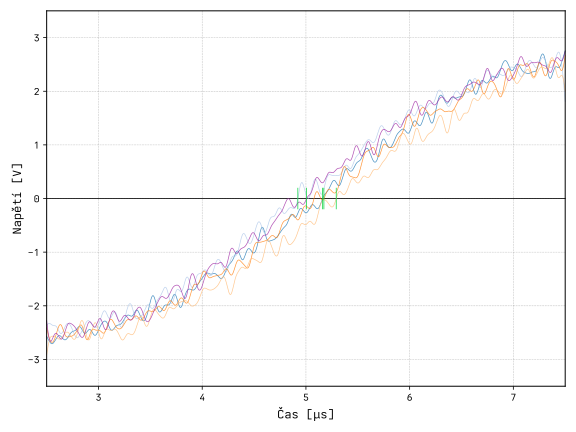
\includegraphics[width=0.8\textwidth]{obrazky/zerocross_noise_chart.pdf} % Adjusted width for the second figure
    \caption{Graf částí zašuměných sinusových signálů s vyznačenými průchody nulou}
    \label{fig:chart_zerocross} % Changed label for the second figure
\end{figure}


\section{Metoda vzorkování a digitálního zpracování}
Alternativou k analogovému převodu na stejnosměrná napětí je přímé vzorkování harmonických signálů pomocí \acs{A/D} převodníku a následné digitální 
zpracování v mikrokontroléru.
Tímto přístupem se lze vyhnout mnoha nedostatkům výše popsané metody.

\subsection{Vzorkování \acs{A/D} převodníkem}

Pro správné vzorkování signálu je nutné dodržet Nyquistův-Shannonův teorém, který říká, že vzorkovací frekvence $f_vz$ musí být alespoň dvojnásobkem nejvyšší frekvence v signálu $f_{max}$:
\begin{equation}
    f_vz \geq 2 \cdot f_{max}
    \label{eq:nyquist}
\end{equation}

V praxi se však používá vzorkovací frekvence výrazně vyšší, typicky 10 až 20 násobek frekvence měřeného signálu, aby bylo zajištěno dostatečné množství vzorků
pro přesné zpracování a potlačení vlivu šumu.

Při nedostatečné vzorkovací frekvenci dochází k jevu zvanému aliasing, kdy se vyšší frekvence v signálu projeví jako nižší frekvence v navzorkovaném signálu. 
Tomu lze předejít použitím antialiasingového filtru před \acs{A/D} převodníkem, který odstraní frekvence vyšší než $f_s/2$.

Vzorkovány jsou dva signály -- napětí a proud. Je důležité, aby byly oba kanály vzorkovány synchronně, 
aby nedošlo k fázovému posunu způsobenému časovým zpožděním mezi vzorky. Toho lze docílit použitím dvou \acs{A/D} převodníků pracujících současně.

\subsection{Výpočet efektivní hodnoty navzorkovaného signálu}
Před výpočtem amplitudy musí být navzorkovaný signál očištěn od případné stejnosměrné složky.
To se provede výpočtem průměrné hodnoty všech vzorků podle vztahu \ref{eq:dc_component}, 
která je následně od každého vzorku odečtena (vztah \ref{eq:remove_dc}).
\begin{equation}
    U_{DC} = \frac{1}{N}\sum_{i=1}^{N} u_i
    \label{eq:dc_component}
\end{equation}
\begin{equation}
    u_{i,AC} = u_i - U_{DC}
    \label{eq:remove_dc}
\end{equation}
kde $N$ je počet vzorků, $u_i$ jsou původní hodnoty napětí a $u_{i,AC}$ jsou hodnoty napětí bez stejnosměrné složky.

Efektivní hodnota \acs{RMS} je obecně definována vztahem:
\begin{equation}
    U_{RMS} = \sqrt{\frac{1}{T}\int_0^T u^2(t) \ dt}
    \label{eq:rms}
\end{equation}
kde $T$ je perioda signálu nebo časový interval, přes který se integruje. \\
Pro její výpočet ze vzorků použijeme diskrétní podobu vztahu \ref{eq:rms_discrete}:

\begin{equation}
    U_{RMS} = \sqrt{\frac{1}{N}\sum_{i=1}^{N} u_i^2}
    \label{eq:rms_discrete}
\end{equation}
kde $N$ je počet vzorků a $u_i$ jsou jednotlivé hodnoty napětí.

Pro harmonický signál s amplitudou $U_m$ platí vztah mezi efektivní hodnotou a amplitudou:
\begin{equation}
    U_{RMS} = \frac{U_m}{\sqrt{2}}
    \label{eq:rms_amplitude}
\end{equation}

Pro potlačení vlivu šumu se často používá průměrování přes více period signálu. Pokud je vzorkováno $M$ period, efektivní hodnota se vypočítá jako:
\begin{equation}
    U_{RMS} = \sqrt{\frac{1}{M \cdot N_p}\sum_{j=1}^{M}\sum_{i=1}^{N_p} u_{i,j}^2}
    \label{eq:rms_averaged}
\end{equation}
kde $N_p$ je počet vzorků v jedné periodě.

\subsection{Výpočet fázového posunu navzorkovaných signálů}

Pro výpočet fázového posunu mezi dvěma navzorkovanými signály existuje několik algoritmů. Jednou z nejpřesnějších metod je výpočet pomocí vzájemné korelace (\acs{cross-correlation}).

Vzájemná korelace dvou signálů $u_1(t)$ a $u_2(t)$ je definována jako:
\begin{equation}
    R_{12}(\tau) = \frac{1}{T}\int_0^T u_1(t) \cdot u_2(t+\tau) \ dt
    \label{eq:crosscorr_cont}
\end{equation}

Pro diskrétní vzorky se vzájemná korelace počítá jako:
\begin{equation}
    R_{12}[k] = \frac{1}{N}\sum_{i=0}^{N-1} u_1[i] \cdot u_2[i+k]
    \label{eq:crosscorr_disc}
\end{equation}

Fázový posun $\varphi$ se získá z časového posunu $\tau_{max}$, při kterém vzájemná korelace dosahuje maxima:
\begin{equation}
    \varphi = 2\pi f \cdot \tau_{max} \quad [\text{rad}]
    \label{eq:phase_from_crosscorr}
\end{equation}
nebo v stupních:
\begin{equation}
    \varphi = 360^\circ \cdot f \cdot \tau_{max} \quad [^\circ]
    \label{eq:phase_from_crosscorr_deg}
\end{equation}

Další možností je použití diskrétní Fourierovy transformace (\acs{DFT}) nebo rychlé Fourierovy transformace (\acs{FFT}). Pokud jsou signály harmonické s frekvencí $f$, lze vypočítat jejich komplexní amplitudy pomocí \acs{DFT}:
\begin{equation}
    U_1 = \frac{2}{N}\sum_{i=0}^{N-1} u_1[i] \cdot e^{-j2\pi f i/f_s}
    \label{eq:dft_u1}
\end{equation}
\begin{equation}
    U_2 = \frac{2}{N}\sum_{i=0}^{N-1} u_2[i] \cdot e^{-j2\pi f i/f_s}
    \label{eq:dft_u2}
\end{equation}

Fázový posun se pak vypočítá z argumentu podílu komplexních amplitud:
\begin{equation}
    \varphi = \arg\left(\frac{U_2}{U_1}\right) = \arg(U_2) - \arg(U_1)
    \label{eq:phase_from_dft}
\end{equation}

Výhodou metody založené na \acs{DFT} je možnost současného výpočtu amplitudy i fáze signálu. Navíc tato metoda lépe potlačuje harmonické složky a šum, pokud je použito okénkování (\acs{windowing}) před transformací.

Pro přesné měření fáze je důležité, aby oba signály byly vzorkovány synchronně a aby byla známa přesná frekvence měřeného signálu. V případě, že frekvence není přesně známa, lze ji odhadnout z navzorkovaných dat pomocí metody nulových průchodů nebo spektrální analýzy.
